\documentclass{article}

\usepackage[francais]{babel}
\usepackage[T1]{fontenc}
\usepackage{moreverb}       % verbatim with tab

\usepackage{wrapfig}
\usepackage{graphicx}
\usepackage{geometry}
\geometry{hmargin=2.5cm}
\usepackage{amsmath}
\usepackage{siunitx}

\usepackage{graphicx}
\usepackage{subcaption}
\usepackage{float}
\usepackage{hyperref}
\usepackage{setspace}
\usepackage{xcolor}
\usepackage{pdfpages}
\usepackage{enumitem}
\usepackage{lscape}

% https://tug.org/FontCatalogue/libertinusserif/
%\usepackage{libertinus}
%\usepackage[T1]{fontenc}

\usepackage{libertine} % Police Linux Libertine en sérif, Linux Biolinum en sans-sérif.

\usepackage[libertine]{newtxmath} % Math avec la police Libertine
%\addtokomafont{disposition}{\normalfont\sffamily} % Police des titres (ajouter \normalfont pour enlever le bold)
%\addtokomafont{paragraph}{\bfseries} % Titre des paragraphes en gras
%\addtokomafont{subsubsection}{\bfseries} % Titre des subsubsections en gras
%\usepackage[scaled=.8]{beramono} % Police monospace

\usepackage{fancyhdr}       % en-têtes
\usepackage{lastpage}       % numéro de dernière page

\title{Développement d'une solution de software embarqué sur processeur ARM pour encodage audio AAC optimisé aux applications d'EVS}
\date{2020 -- 2021}
\author{Laura Binacchi}

\pagestyle{fancy}
\renewcommand\headrulewidth{1pt}
\fancyhead[L]{Laura Binacchi}
\fancyhead[C]{Programmation procédurale}
\fancyhead[R]{\today}

\AtBeginDocument{
    \def\labelitemi{\textbullet}    % Redéfinition des puces dans les itemize
    \renewcommand{\times}{\text{×}} % Remplacer le gros «X» par un plus beau
    %\interfootnotelinepenalty=10000
}

\begin{document}
    \pagenumbering{gobble}
    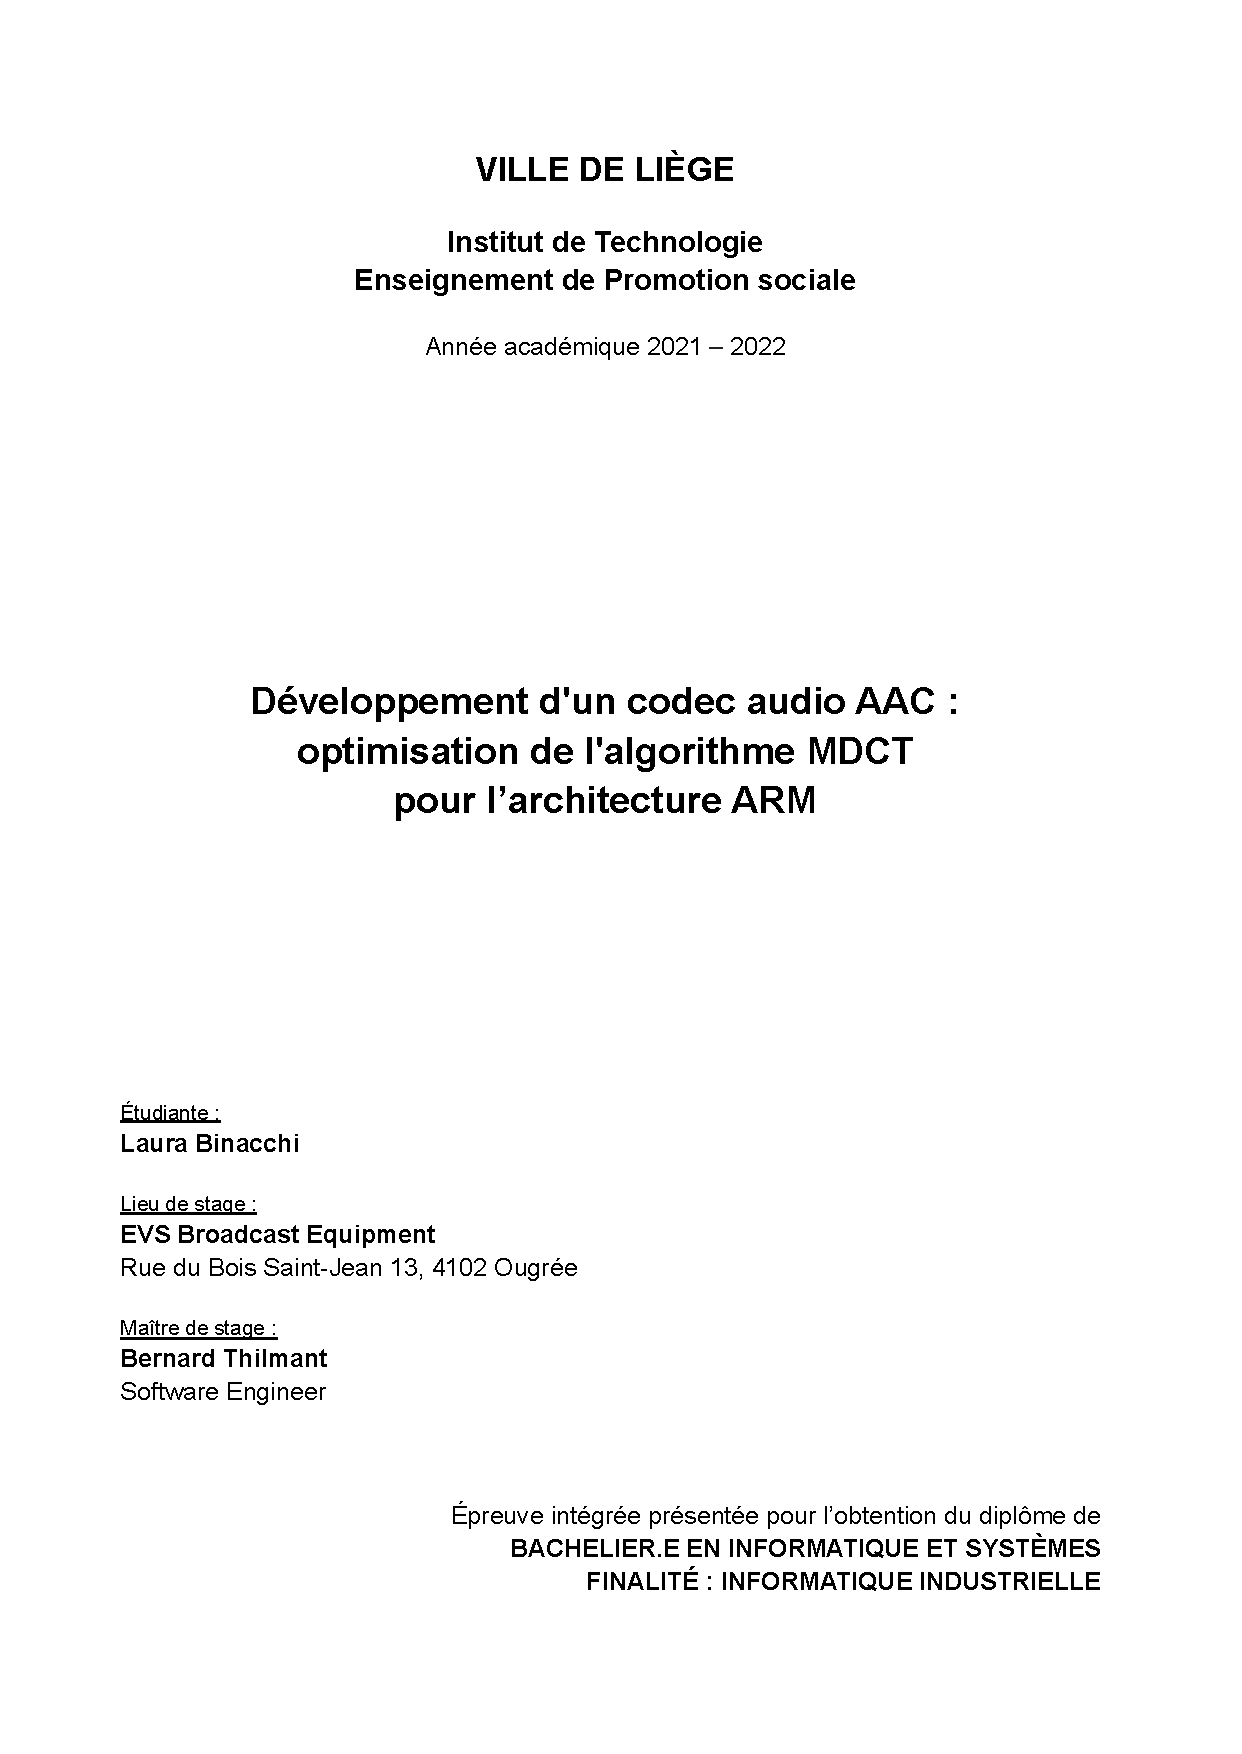
\includepdf[pages={1}]{pdg}
    \newpage
    \tableofcontents
    \newpage
    \pagenumbering{arabic}

    \section*{Remerciements}
    \paragraph{}

    \section*{Introduction}
    \paragraph{}
    Développement d'une solution de software embarqué sur processeur ARM pour encodage audio AAC optimisé aux applications d'EVS :
    \begin{itemize}
        \item Prise de connaissance de l'encodage AAC et de l'environnement EVS qui utilise ce type de format ;
        \item Prise de connaissance des résultats des optimisations possibles du modèle psycho-acoustique développé par EVS ;
        \item Développement du code en C ou Assembler pour l'encodage AAC sur plateforme ARM ;
        \item Test du système et documentation de son implémentation.
    \end{itemize}

    \section{Le signal audio : généralités}

    onde acoustique -> 

    - son audible = vibration entre 20 et 20kHz

    le signal, analogique (continu) ou discret, peut avoir une représentation :
    - temporelle
    - fréquentielle
    exemple de signaux périodiques (sinus, carré, etc) -> pp 6-7 + truc interactif

    - spectre d'amplitude (utile) et spectre de phase (pas utile)

    - toute fonction p(x, t) peut être exprimée par une somme de fonctions (co-)sinusoidales : formule pour les fonctions périodiques + transformée de Fourier pour les fonctions n'est pas périodique dans le temps


    \section{Les codecs audio}
    \section{Les normes MPEG}
    \section{Les différents blocs qui composent un encodeur audio (et un décodeur pour info/symétrie ?)}v
    
    \section{Transformation de Fourier}
    Dans les généralités ??
    % https://www.claudegabriel.be/Math%C3%A9matiques%20appliqu%C3%A9es,%20chapitre%204.pdf -> p12 sur N pair / impair
    % à la base -> signaux périodique (faire bref)
    
    % -> ce qui nous intéresse : transformation pour signal non périodique discret -> DCT

    \section{FFT}
    \url{https://infoscience.epfl.ch/record/59946}
    \url{https://www.cis.rit.edu/class/simg716/Gauss_History_FFT.pdf}
    \url{https://sci-hub.se/https://www.jstor.org/stable/29775194#}

    \section{MDCT}
    \begin{itemize}
        \item particularités par rapport à la FFT
        \item basée sur la DCT-IV
        \item niveaux de complexité (O...)
    \end{itemize}

    \section{Optimisations du bloc MDCT}
    \begin{itemize}
        \item utilisation d'un algorithme FFT optimisé pour architecture ARM
        \item optimisations MDCT (pre et post processing/twiddles pour faire moins de FFT) -> réduction de la fenêtre de la FFT
    \end{itemize}

    \subsection{FFT de Ne10}

    \subsubsection{Validation des données de sortie}
    \begin{itemize}
        \item sortie des données et générations de graphiques avec gnuplot
        \item résolution en fréquence pour une fenetre de 64 samples : période de 2 pi -> 64 samples -> signal échantillonné à 48kHz -> 1.3333... ms -> f = 1 / 1.33333 = 750 Hz OU res = fs / samples -> sur les graphiques on a des raies de fréquence de 750 Hz
    \end{itemize}

    Graphiques sur sinusoide simple : augmenter la fréquence (i * qch pour déplacer la bande de fréquence), 

    \subsection{Code MDCT sur algo FFT}
    \begin{itemize}
        \item fenêtre de 1024
        \item pre-twiddle -> 256
        \item FFT
        \item post-twiddle -> 512
    \end{itemize}
    
    \paragraph{Rem} trivial en float (reprendre le code de dsp) mais pour l'implémentation en arithmétique entière, attention à mettre dans les bonnes ranges

    \paragraph{}
    Optimisations :
    \begin{itemize}
        \item jouer sur la symétrie pour ne calculer que la moitié
        \item 
    \end{itemize}

    \paragraph{Tests}
    Réaliser une fonction qui calcule la somme des cosinus (formule de wikipedia) pour chaque samples (pas du tout optimisée donc super lente). Pour la calcul en integer, on peut autoriser un manque de précision de max 1 LSB.

    \paragraph{Points d'attention}
    \begin{itemize}
        \item les dépassements : 16 bits + 32 bits -> potentiellement 33 bits, 16*16 -> 32, etc. à voir en fonction des valeurs réelles
        \item alignement des tableaux (souvent c'est une contrainte imposée car permet facilement d'optimiser du code) : résolutions possibles en allouant dynamiquement les tableaux et en jouant avec une arithmétique de pointeur OU utilisation de posix mem align...
    \end{itemize}



    \section*{Conclusion}
    \paragraph{}

\end{document}